\documentclass[11pt,a4paper]{article}
\usepackage[margin=1.5cm,top=1.3cm,bottom=1.3cm]{geometry}
\usepackage{amsmath,amssymb}
\usepackage{graphicx}
\usepackage{booktabs}
\usepackage{hyperref}
\usepackage{xcolor}
\usepackage{caption}
\usepackage{subcaption}

\hypersetup{colorlinks=true,linkcolor=blue,citecolor=blue,urlcolor=blue}
\setlength{\abovedisplayskip}{4pt}\setlength{\belowdisplayskip}{4pt}
\setlength{\abovedisplayshortskip}{2pt}\setlength{\belowdisplayshortskip}{2pt}
\captionsetup{skip=3pt,font=small}
\setlength{\floatsep}{6pt}\setlength{\textfloatsep}{7pt}\setlength{\intextsep}{6pt}
\setlength{\parskip}{2pt}\setlength{\parindent}{0pt}

\title{\vspace{-1.2em}\textbf{Final Project: 3-D Reconstruction from a Slit-Laser
       Turntable Scanner via Triangulation}}
\author{Student ID: M11415015}
\date{2026 Spring --- Computer Vision and Applications}

\begin{document}
\maketitle
\vspace{-2.2em}

% ───────────────────────────────────────────────────────────────────────────
\section{Problem and Coordinate Frame}
% ───────────────────────────────────────────────────────────────────────────
A green slit laser projects a vertical plane that passes through the rotation
axis of a hexagonal turntable. A fixed camera captures the scene while the table
(and the gnome on it) rotate in $2^\circ$ steps, giving $180$ frames over
$360^\circ$ in two sets: \texttt{withLaser} and \texttt{withoutLaser}
($720\times1280$). The goal is one coloured 3-D point cloud.

\textbf{World frame.} Origin at the turntable centre, $+Z$ = rotation axis (up).
From \texttt{GroundTruth.ply} the turntable is a regular hexagonal prism of
circum-radius $R=25$\,mm (vertex--vertex diameter $50$\,mm), top face $z=+1$,
bottom $z=-14$ (thickness $15$\,mm). Reconstruction is performed in this frame;
\texttt{GroundTruth.ply} is used \emph{only} for the final error analysis.

The pipeline is the classical laser-plane triangulation: each laser pixel
back-projects to a camera ray which is intersected with the (calibrated) laser
plane to give a 3-D point; points are then de-rotated by the frame angle and
accumulated.

% ───────────────────────────────────────────────────────────────────────────
\section{Camera Calibration (Extrinsics and Focal)}
% ───────────────────────────────────────────────────────────────────────────
A world point $\mathbf{P}$ projects as $s[u,v,1]^\top=K[R\,|\,\mathbf{t}]\,
[\mathbf{P},1]^\top$. We recover $\{R,\mathbf t\}$ from the turntable, whose
metric geometry is known. In \texttt{withoutLaser/0000.jpg} the prism silhouette
is segmented (bright, low saturation) and six corners are located sub-pixel by
intersecting line-fits of the silhouette edges (Table~\ref{tab:corners}). These
are matched to the hexagon vertices (one near vertex with both side vertical
edges visible $\Rightarrow$ three consecutive vertices) and the pose is solved
with \texttt{cv2.solvePnP}.

\textbf{Focal correction.} The nominally provided $f=720$\,px is \emph{not}
consistent with the imaged $50$\,mm turntable (best reprojection $>22$\,px at any
pose). Refining $f$ together with the pose gives $f\!\approx\!1281$\,px
($=720\times16/9$, a render FOV/sensor-fit artefact) and a reprojection RMS of
\textbf{0.04\,px}; the principal point $(c_x,c_y)=(360,640)$ is the image centre
and checks out exactly. We therefore adopt
\[
  K=\begin{bmatrix}1281 & 0 & 360\\ 0 & 1281 & 640\\ 0&0&1\end{bmatrix},\qquad
  \mathbf{C}=-R^\top\mathbf t=(-112.6,\,10.8,\,25.4)\ \text{mm},
\]
i.e.\ camera distance $116$\,mm, azimuth $174.5^\circ$, elevation $12.7^\circ$.
The world-frame azimuth is a free gauge (fixed by placing one vertex at
$90^\circ$); the table's true frame-0 azimuth becomes a global yaw vs.\ the
ground truth and is irrelevant to shape.

\begin{table}[h]
\centering\footnotesize
\caption{Six turntable corners on frame 0 and per-corner reprojection error
($f{=}1281$). Mean RMS $=0.04$\,px, max $=0.10$\,px.}
\label{tab:corners}
\setlength{\tabcolsep}{4pt}
\begin{tabular}{lcccccc}
\toprule
corner & A$_{\text{top}}$ & A$_{\text{bot}}$ & B$_{\text{near}}$ & C$_{\text{bot}}$ & C$_{\text{top}}$ & D$_{\text{top}}$\\
\midrule
$(u,v)$ px & (84,921) & (84,1095) & (224,1198) & (572,1184) & (572,977) & (648,911)\\
err (px)   & 0.10 & 0.07 & 0.03 & 0.03 & 0.02 & 0.01\\
\bottomrule
\end{tabular}
\end{table}

% ───────────────────────────────────────────────────────────────────────────
\section{Laser-Plane Estimation}
% ───────────────────────────────────────────────────────────────────────────
Because the beam passes through the rotation axis, the laser plane contains the
$z$-axis: $a\,x+b\,y=0$. We isolate the stripe that lands on the \emph{bare}
turntable top face ($z=+1$) over the first frames (inside the projected top
hexagon, on the bright table only), back-project each pixel to $z=+1$, and fit a
line through the origin. From $948$ points:
\[
  -0.504\,x-0.864\,y=0\quad(\text{residual RMS}=0.30\,\text{mm}).
\]
Figure~\ref{fig:calib} overlays the reprojected prism wireframe and this plane
on the scan, confirming the calibration.

% ───────────────────────────────────────────────────────────────────────────
\section{Stripe Detection and Triangulation}
% ───────────────────────────────────────────────────────────────────────────
\textbf{Detection.} Per frame, the excess-green response
$\text{resp}=2G-R-B$ of $(\text{withLaser}-\text{withoutLaser})$ isolates the
stripe (Fig.~\ref{fig:laser}). The green laser is largely absorbed by the
\emph{red} hat, so $G-\max(R,B)$ detects only $\sim$50\% of the hat rows (a hole
at the tip); the excess-green index is far more sensitive there ($\sim$64\% at
the same threshold) while keeping a $0\%$ background false-positive rate. Per
image row the stripe column is the intensity-weighted centroid around the peak
(sub-pixel, $\pm5$\,px window, threshold $35$).

\textbf{Triangulation.} For pixel $(u,v)$ the world ray is
$\mathbf d=R^\top K^{-1}[u,v,1]^\top$ from $\mathbf C$; intersecting
$a x+b y=0$ gives $s=-(aC_x+bC_y)/(a d_x+b d_y)$ and
$\mathbf X=\mathbf C+s\,\mathbf d$. Colour is bilinearly sampled from
\texttt{withoutLaser} (no green tint).

\textbf{Rotation direction (image-only).} Tracking the near-vertex azimuth shows
it increases $+2^\circ$/frame, so the table turns CCW about $+z$; a point seen at
frame $i$ is de-rotated by $R_z(-2^\circ i)$ into the frame-0 object frame and
accumulated. The cloud is then cropped to the scan volume ($r\le26$\,mm),
down-sampled to a $0.4$\,mm voxel grid, and cleaned by a $k$-NN distance test
plus a radius-outlier test (which removes the faint laser spray above the hat
tip). Result: $160{,}037\to42{,}341$ coloured points (Fig.~\ref{fig:recon}).

\begin{figure}[t]
\centering
\begin{subfigure}{0.20\textwidth}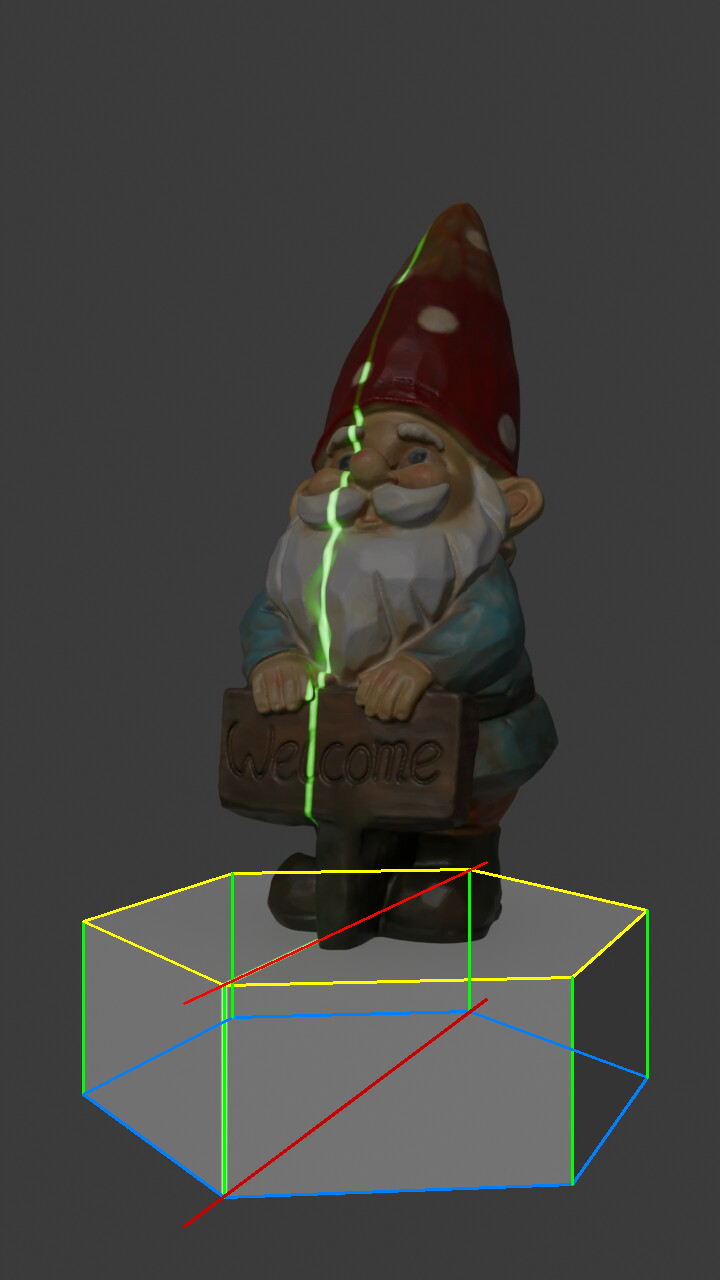
\includegraphics[width=\linewidth]{figs/calib.png}
\caption{}\label{fig:calib}\end{subfigure}\hfill
\begin{subfigure}{0.40\textwidth}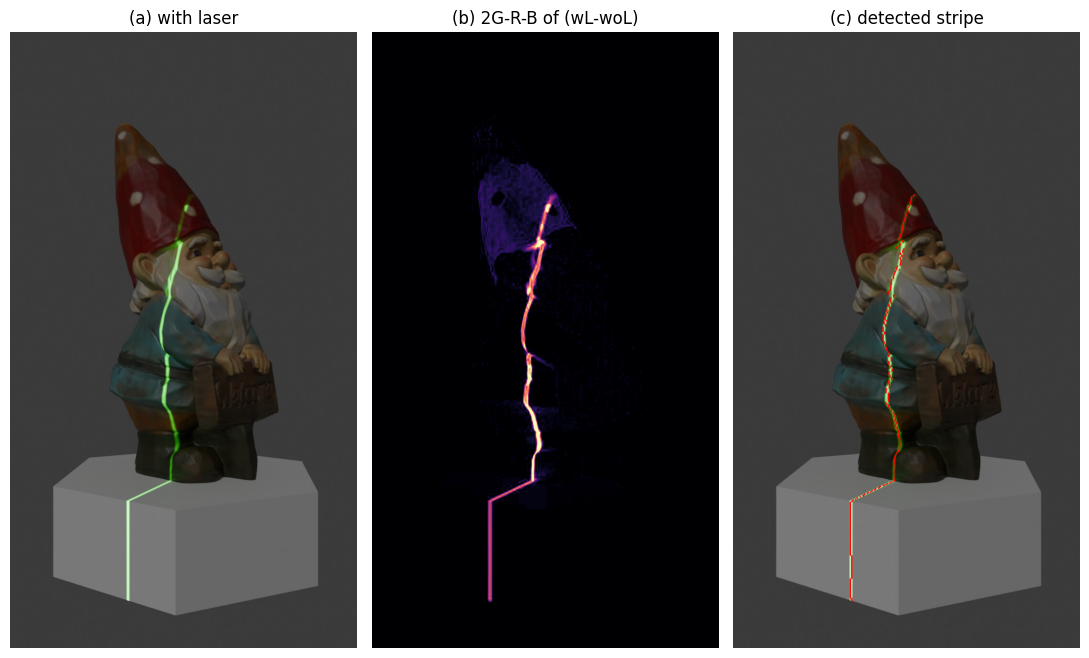
\includegraphics[width=\linewidth]{figs/laser.png}
\caption{}\label{fig:laser}\end{subfigure}\hfill
\begin{subfigure}{0.37\textwidth}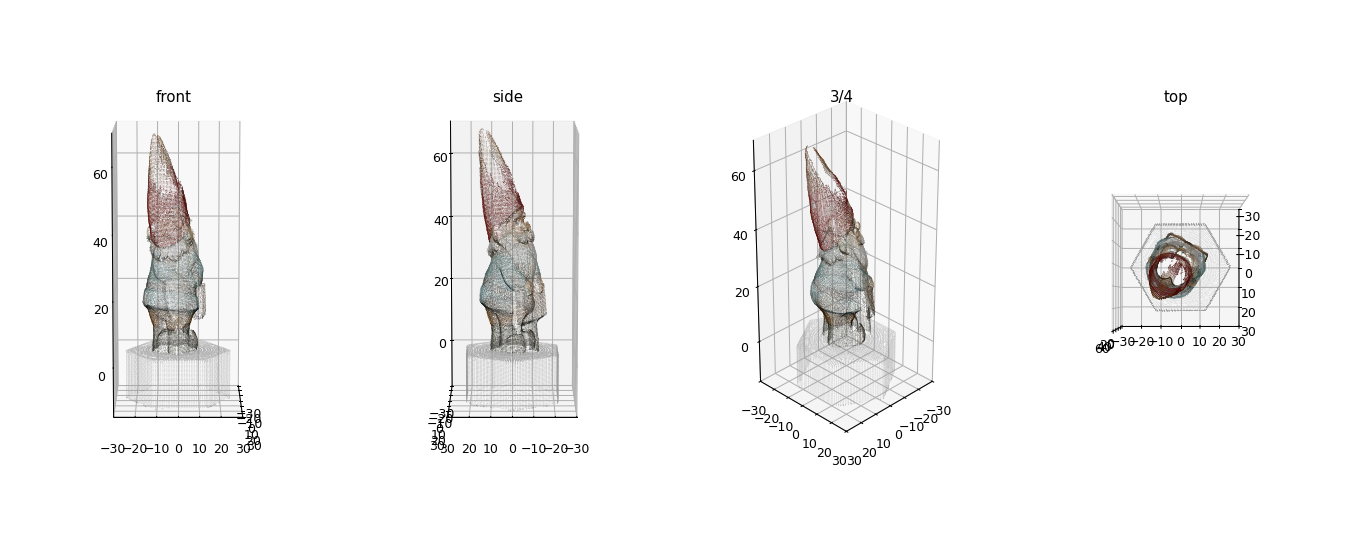
\includegraphics[width=\linewidth]{figs/recon.png}
\caption{}\label{fig:recon}\end{subfigure}
\caption{(a) Calibration overlay: reprojected prism (yellow/blue/green) and laser
plane (red) on the scan. (b) Stripe detection: with-laser, $2G-R-B$
response, and detected sub-pixel stripe (red). (c) Reconstructed coloured cloud
(42{,}341 pts) -- front, side, 3/4, top.}
\end{figure}

% ───────────────────────────────────────────────────────────────────────────
\section{Results and Error Analysis}
% ───────────────────────────────────────────────────────────────────────────
The cloud is compared to a dense ($4\times10^5$ pts) area-weighted sampling of
the GT mesh. Sharing origin, scale and $z$-axis with the GT, the only free DOF is
a yaw; a $1^\circ$ yaw search ($300^\circ$, no mirror $\Rightarrow$ handedness
correct) plus a few rigid-ICP steps aligns them (this alignment is an
evaluation-only diagnostic). Distances are reported both ways
(Table~\ref{tab:err}, Figs.~\ref{fig:hist}--\ref{fig:emap}).

\begin{table}[h]
\centering\footnotesize
\caption{Cloud-to-cloud distances (mm). recon$\to$GT = accuracy;
GT$\to$recon = coverage.}
\label{tab:err}
\setlength{\tabcolsep}{6pt}
\begin{tabular}{lccccc}
\toprule
direction & mean & median & RMS & 95\% & max\\
\midrule
recon $\to$ GT (accuracy) & 0.203 & \textbf{0.180} & 0.244 & 0.424 & 2.55\\
GT $\to$ recon (coverage) & 1.48 & 0.30 & 3.41 & 9.09 & 16.9\\
\bottomrule
\end{tabular}
\end{table}

\begin{figure}[h]
\centering
\begin{subfigure}{0.46\textwidth}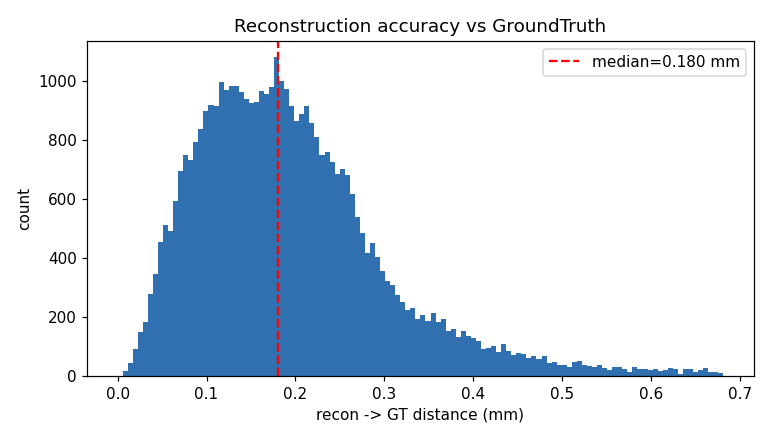
\includegraphics[width=\linewidth]{figs/hist.png}
\caption{}\label{fig:hist}\end{subfigure}\hfill
\begin{subfigure}{0.50\textwidth}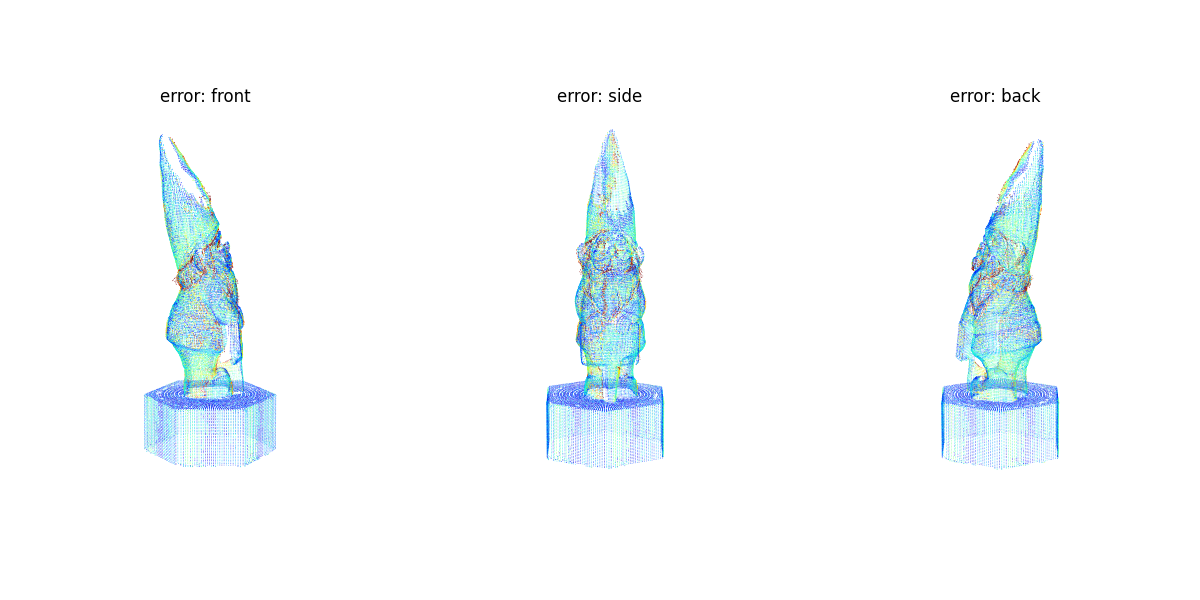
\includegraphics[width=\linewidth]{figs/errormap.png}
\caption{}\label{fig:emap}\end{subfigure}
\caption{(a) Histogram of recon$\to$GT distance. (b) Error map (jet: blue
$0$\,mm $\to$ red $\ge0.5$\,mm); most of the surface is sub-$0.2$\,mm, with
larger error only at steep edges/fine detail.}
\end{figure}

\textbf{Accuracy} is excellent: median $0.18$\,mm and $95\%$ below $0.44$\,mm,
i.e.\ well under $1\%$ of the object size, consistent with the $0.04$\,px
calibration and $0.30$\,mm plane fit. The error map shows the largest residuals
on steep/oblique surfaces (hat sides, beard, sign edges) where the stripe
centroid is least precise.

\textbf{Coverage.} $78.3\%$ of the GT lies within $1$\,mm of a reconstructed
point. The uncovered $\sim$22\% (long GT$\to$recon tail) are regions a single
fixed camera+laser cannot see: deep concavities, surfaces between the legs and
under the welcome sign/arms, and the turntable underside. These are intrinsic
occlusions of the setup, not calibration error -- accuracy where the laser
\emph{is} seen remains sub-millimetre.

\textbf{Conclusion.} A fully image-derived calibration (PnP on the known
turntable, focal corrected to $1281$\,px, $z$-axis laser plane) plus background-
subtraction stripe detection and ray--plane triangulation reconstructs the gnome
to a median accuracy of $0.18$\,mm. Deliverables: \texttt{calibrate.py},
\texttt{reconstruct.py}, \texttt{error\_map.py}, and \texttt{M11415015.xyz}.

\end{document}
